	\section{Le générateur}
	Comme montré dans le schéma \ref{fig:generalDig}, une fois le walkthrough parsé, il faut générer les fichiers nécessaire au test. Pour cela, j'ai créé un \textit{package} de classes ayant des services permettant d'ajouter les fonctionnalités à générer : Ajouter un check, ajouter une affectation, ajouter une action debugger, ajouter les informations des tests, \ldots et lancer la génération du fichier.

		\subsection{Génération des tests}
		Je dois générer 3 types de fichiers : un précondstim, des stimscenarios et un \texttt{GreenTTest} pour chaque test. Chacune des classes que je génères hérite d'une classe présente dans \textit{GreenT}, respectivement \texttt{PrecondStim}, \texttt{StimScenario} et \texttt{GreenTTest}.

		La génération des fichiers possède des points communs en fonction du type de fichier, principalement entre un \texttt{PrecondStim} et un \texttt{StimScenario}, ainsi j'ai conçu un arbre d'héritage assez simple me permettant de factoriser le code : 
		\begin{figure}[H]
		\centering
		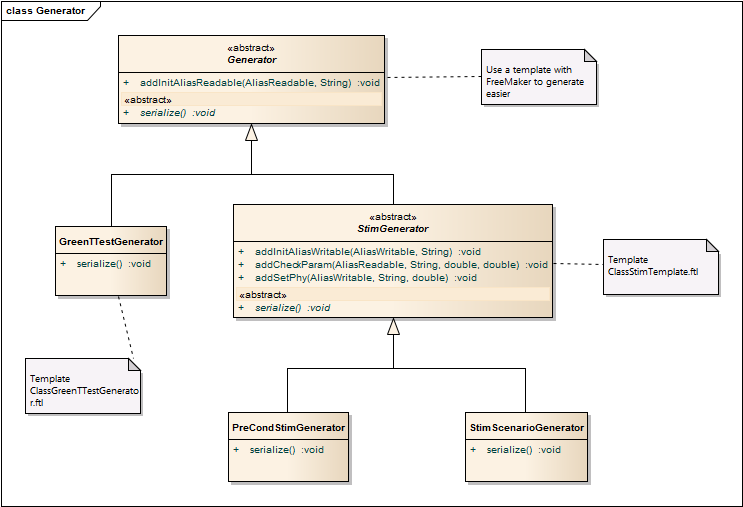
\includegraphics[width=14cm]{contents/images/generatorClass.png}
		\caption{Diagramme de classes du générateur}
		\end{figure}
		La méthode \textit{serialize} écrit le code Java, avant d'appeler cette méthode il est donc nécessaire de << remplir >> l'objet avec les informations nécessaires via les autres méthodes.
		
		\subsection{Le moteur de template : freemarker}
		\begin{wrapfigure}{l}{3cm}
			
\includegraphics[width=3cm]{contents/images/FreeMarker.png}
		\end{wrapfigure}
		Les classes que je génères ont un gabarit commun, seul l'implémentation des méthodes changent, ainsi plutôt que réécrire systématiquement tout le corps de la classe, il parraissait intéressant d'avoir un moteur de \textit{template}, j'ai choisi FreeMarker.

		J'ai un fichier gabarit utilisant le format FreeMarker, avec dedans des appels d'objet. Lors de la sérialisation, je fournis à FreeMarker les objets concernés, l'adresse du gabarit et c'est lui qui écrira le fichier \texttt{.java}.

		Deux fichiers de templates ont été nécessaires : un pour les stim, et un pour le \textit{GreenTTest}. En effet un precondstim et un stimscenario n'ont que peu de différence, il était donc possible de les regrouper avec le même template.

		Le template des stim contient une liste d'actions à exécuter dans la méthode d'exécution, et une liste d'alias nécessaire qui doivent être ajoutés dans une méthode adéquate. \\
		Le template des \textit{GreenTTest} lui contient une méthode permettant de remplir le rapport et une méthode qui créé l'\textit{Expected Behavior}.
		Les deux templates ont également une liste d'import qui est ajoutés automatiquement en début du fichier, ceux-ci sont disponibles dans l'annexe \ref{annexeTemplate} suivis de deux exemples de fichiers générés annexe \ref{annexeGeneration}.

	
		\begin{figure}[H]
		\centering
		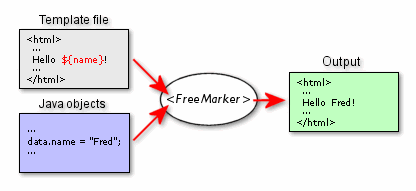
\includegraphics[width=12cm]{contents/images/FreeMarkerSchema.png}
		\caption{Schéma de fonctionnement de FreeMarker}
		\end{figure}
		\begin{remarque}
		Cet exemple qui vient du site officiel de FreeMarker utilise des templates HTML, pour ma part j'ai créé des templates Java, mais le principe est le même.
		\end{remarque}